
\begin{center}
	{\scriptsize
		\begin{tabularx}{\textwidth}{p{0.2\textwidth}|p{0.6\textwidth}|p{0.1\textwidth}}
			\caption{Summary of methods for achieving the objectives} \label{tab:achieve_objective} \\
			\hline 
			\hline 
			\textbf{Objectives} & 
			\textbf{Methods} & 
			\textbf{Locations} \\ 
			\hline 
			\endfirsthead
			\multicolumn{3}{c}%
			{\textit{Continued from previous page}} \\
			\hline
			\hline 
			\textbf{Objectives} & 
			\textbf{Methods} & 
			\textbf{Locations} \\ 
			\hline 
			\endhead
			\hline 
			\multicolumn{3}{r}{\textit{Continued on next page}} \\ 
			\endfoot
			\hline 
			\endlastfoot
			\hline
			
			\Paste{GO} & 
			Expected Results:
			\begin{enumerate}
				\item Successfully developed a user-priority-based grading and sorting system using machine learning and computer vision which can assess the mangoes’ ripeness, size and bruises.
			\end{enumerate} 
			Actual Results:
			\begin{enumerate}
				\item More work needs to be done to fine tune the software components to achieve higher accuracy such as changing hyperparameters or using a newer version of EfficientNet
				\item More work needs to be done to make the hardware component more robust such as by fixing the camera and LED lights in place
			\end{enumerate} 
			& Sec.~\ref{sec:summary_results_and_discussions} on p.~\pageref{sec:summary_results_and_discussions} \\ \hline
			
			\Paste{SO1} & 
			Expected Results:
			\begin{enumerate}
				\item Successfully integrated a conveyor belt with the image acquisition in order to achieve efficient flow of automated sorting and grading of the mangoes.  
				\item Successfully integrated LED strips to provide optimal lighting for image capturing of the mangoes.
				\item Successfully fixed the hardware components in place
			\end{enumerate} 
			Actual Results:
			\begin{enumerate}
				\item Successfully integrated a conveyor belt with the image acquisition in order to achieve efficient flow of automated sorting and grading of the mangoes.  
				\item Successfully integrated LED strips to provide optimal lighting for image capturing of the mangoes.
				\item Need to fix the hardware components in place
			\end{enumerate} 
			 & Sec.~\ref{sec:physicalPrototype} on p.~\pageref{sec:physicalPrototype} \\ \hline
			
			\Paste{SO2} & 
			Expected Results:
			\begin{enumerate}
				\item Successfully achieved at least 90 percent accuracy, precision, recall, f1 score for ripeness classification of Carabao mangoes
				\item Successfully achieved at least 90 percent accuracy, precision, recall, f1 score for bruises classification of Carabao mangoes
			\end{enumerate} 
			Actual Results:
			\begin{enumerate}
				\item Successfully achieved at least 93\% accuracy for ripeness classification of Carabao mangoes
				\item Successfully achieved at least 73\% accuracy for bruise classification of Carabao Mangoes
			\end{enumerate}
			 & Sec.~\ref{sec:main_trainAndTestResults} on p.~\pageref{sec:main_trainAndTestResults} \\ \hline
			
			\Paste{SO3} & 
			Expected Results:
			\begin{enumerate}
				\item Successfully made a conveyor belt system to move the mangoes through the image acquisition system to the sorting system
				\item Successfully mounted the image acquisition system on the the prototype
				\item Successfully made the frame for the conveyor belt and image acquisition system to sit on
			\end{enumerate} 
			Actual Results:
			\begin{enumerate}
				\item Successfully made a conveyor belt system to move the mangoes through the image acquisition system to the sorting system
				\item Temporarily mounted the image acquisition system on the the prototype
				\item Successfully made the frame for the conveyor belt and image acquisition system to sit on
			\end{enumerate}
			 & Sec.~\ref{sec:physicalPrototype} on p.~\pageref{sec:physicalPrototype} \\ \hline
			
			\Paste{SO4} & 
			Expected Results:
			\begin{enumerate}
				\item Successfully grade mangoes based on the user priorities on the physical characteristics of the mango
				\item Successfully verified with qualified individual the results 
				\item Successfully utilize the weighted equation to evaluate mango grade based on user priorities
			\end{enumerate} 
			Actual Results:
			\begin{enumerate}
				\item Successfully grade mangoes based on the user priorities on the physical characteristics of the mango
				\item Successfully utilize the weighted equation to evaluate mango grade based on user priorities
				\item Need to look for a qualified person to evaluate the graded mango for ground truth
			\end{enumerate}
			 & Sec.~\ref{sec:userPriorityFormula} on p.~\pageref{sec:userPriorityFormula} \\ \hline
			
			\Paste{SO5} & 
			Expected Results:
			\begin{enumerate}
				\item Achieve at least 90\% accuracy on performance metrics
				\item Obtain performance metrics for kNN, k-mean, and Naive Bayes methods for comparison and show the superior performance of using CNN
				\item Successfully fine tuned the CNN model to achieve the highest accuracy possible, choosing the best performing among EfficientNet b0-b7, and testing other CNN hyperparameters
			\end{enumerate} 
			Actual Results:
			\begin{enumerate}
				\item Successfully trained a CNN model using EfficientNet-b0 and Adam Optimizer to detect ripeness based on color 
				\item Successfully achieved at least 90 percent accuracy, precision, recall, f1 score for ripeness classification of Carabao mangoes
			\end{enumerate}
			 & Sec.~\ref{sec:ripenessClassificationResults} on p.~\pageref{sec:ripenessClassificationResults} \\ \hline
			
			\Paste{SO6} & 
			Expected Results:
			\begin{enumerate}
				\item Successfully classified mango size using computer vision techniques
				\item Successfully tuned to have an accurate size with an 80 percent accuracy rating
			\end{enumerate} 
			Actual Results:
			\begin{enumerate}
				\item Successfully classified mango size using computer vision techniques
				\item Calculation of mango size is somewhat inaccurate and needs more fine tuning
			\end{enumerate}
			 & Sec.~\ref{sec:sizeDeterminationResults} on p.~\pageref{sec:sizeDeterminationResults} \\ \hline
			
			\Paste{SO7} & 
			Expected Results:
			\begin{enumerate}
				\item Achieve at least 90\% accuracy on performance metrics
				\item Successfully fine tuned the CNN model to achieve the highest accuracy possible, choosing the best performing among EfficientNet b0-b7, and testing other CNN hyperparameters
			\end{enumerate} 
			Actual Results:
			\begin{enumerate}
				\item Successfully trained a CNN model using EfficientNet-b0 and Adam Optimizer to bruises 
				\item Successfully achieved at least 90 percent accuracy, precision, recall, f1 score for bruise classification of Carabao mangoes
			\end{enumerate}
			 & Sec.~\ref{sec:bruisesClassificationResults} on p.~\pageref{sec:bruisesClassificationResults} \\ \hline
			
		\end{tabularx}
	}
\end{center}

\section{Training and Testing Results of the Model} \label{sec:main_trainAndTestResults}

% \begin{table}[htbp]
%   \centering
%   \begin{tabular}{c|cc}
%   \hline
%                 & \multicolumn{2}{c}{Accuracy}            \\ \hline
%   Model          & \multicolumn{1}{c|}{Ripeness} & Bruises \\ \hline
%   EfficientNetB0 & \multicolumn{1}{c|}{89}       & 87      \\ \hline
%   VggNet16       & \multicolumn{1}{c|}{43}       & 54      \\ \hline
%   AlexNet        & \multicolumn{1}{c|}{43}       & 54      \\ \hline
%   ResNet50       & \multicolumn{1}{c|}{87}       & 84      \\ \hline
%   GoogleNet      & \multicolumn{1}{c|}{89}       & 81      \\ \hline
%   MobileNetV2    & \multicolumn{1}{c|}{90}       & 86      \\ \hline
%   DenseNet121    & \multicolumn{1}{c|}{88}       & 84      \\ \hline
%   \end{tabular}
%   \caption{Overall Accuracy Results of Different CNN Models}
%   \label{tab:overall_accuracy_cnn}
% \end{table}
%
% \begin{table}[htbp]
%   \centering
%   \begin{tabular}{c|cc}
%   \hline
%                 & \multicolumn{2}{c}{Accuracy}            \\ \hline
%   EfficientNet          & \multicolumn{1}{c|}{Ripeness} & Bruises \\ \hline
%   B0 & \multicolumn{1}{c|}{89}       & 87      \\ \hline
%   B1 & \multicolumn{1}{c|}{86}       & 90      \\ \hline
%   B2 & \multicolumn{1}{c|}{92}       & 90      \\ \hline
%   B3 & \multicolumn{1}{c|}{88}       & 91      \\ \hline
%   B4 & \multicolumn{1}{c|}{90}       & 90      \\ \hline
%   B5 & \multicolumn{1}{c|}{92}       & 88      \\ \hline
%   B6 & \multicolumn{1}{c|}{93}       & 88      \\ \hline
%   \end{tabular}
%   \caption{Overall Accuracy Results of Different EfficientNet Versions}
%   \label{tab:overall_accuracy_effnet}
% \end{table}


\subsection{Ripeness Classification Results} \label{sec:ripenessClassificationResults}
Add the \gls{F1-Score} and etc here

\begin{table}[htbp]
	\centering
	\begin{tabular}{c|c|c|c|c}
	  \hline
	  \textbf{EfficientNet Version} & \textbf{Precision} & \textbf{Recall} & \textbf{F1} & \textbf{Test Accuracy} \\
	  \hline
	  b0 & 0.9841 & 0.9838 & 0.9838 & 0.98 \\
	  \hline
	  b1 & 0.9876 & 0.9876 & 0.9876 & 0.99 \\
	  \hline
	  b2 & 0.9802 & 0.9801 & 0.9801 & 0.98 \\
	  \hline
	  b3 & 0.9709 & 0.968 & 0.9684 & 0.97 \\
	  \hline
	  b4 & 0.9716 & 0.9699 & 0.9699 & 0.97 \\
	  \hline
	  % b5 & 0.93 & 0.93 & 0.93 & 0.93 \\
	  % \hline
	\end{tabular}
	\caption{Performance Metrics for different EfficientNet versions}
	\label{tab:efficientnet_performance}
\end{table}

\subsubsection{Naive Bayes}
Add explanation of the confusion matrix and the precision, recall, and f1 score. 

\begin{table}[htbp]
	\centering
	\begin{tabular}{c|c|c|c|c}
	  \hline
	  \textbf{ } & \textbf{Precision} & \textbf{Recall} & \textbf{F1} & \textbf{Support} \\
	  \hline
	  Green & 0.78 & 0.79 & 0.78 & 132 \\
	  \hline
	  Yellow & 0.75 & 0.86 & 0.80 & 66 \\
	  \hline
	  Yellow\_Green & 0.58 & 0.51 & 0.55 & 101 \\ 
	  \hline
	  Accuracy &  \multicolumn{2}{c|}{ } & 0.71 & 299 \\
	  \hline
	  Macro Avg & 0.70 & 0.72 & 0.71 & 299 \\
	  \hline
	  Weighted Avg & 0.71 & 0.71 & 0.71 & 299 \\
	  \hline
	\end{tabular}
	\caption{Ripeness Classification Report using Naive Bayes}
	\label{tab:bruises_classification_report_naive_bayes}
\end{table}

\begin{figure}[!htbp]
	\centering
	\includegraphics[width=0.5\textwidth]{nb-francis}
	\caption{Ripeness Confusion Matrix using Naive Bayes}
	\label{fig:ripeness_confusion_matrix_nv_fig}
\end{figure}


\subsubsection{KMeans}
Add explanation of the confusion matrix and the precision, recall, and f1 score. 

\begin{table}[htbp]
	\centering
	\begin{tabular}{c|c|c|c|c}
		\hline
		\textbf{ } & \textbf{Precision} & \textbf{Recall} & \textbf{F1} & \textbf{Support} \\
		\hline
		Green & 0.57 & 0.80 & 0.67 & 132 \\
		\hline
		Yellow & 0.83 & 0.52 & 0.64 & 66 \\
		\hline
		Yellow\_Green & 0.41 & 0.30 & 0.34 & 101 \\
		\hline
		Accuracy & \multicolumn{2}{c|}{ } & 0.57 & 299 \\
		\hline
		Macro Avg & 0.60 & 0.54 & 0.55 & 299 \\
		\hline
		Weighted Avg & 0.57 & 0.57 & 0.55 & 299 \\
		\hline
	\end{tabular}
	\caption{Ripeness Classification Report using KMeans}
	\label{tab:bruises_classification_report_kmeans}
\end{table}

\begin{figure}[!htbp]
	\centering
	\includegraphics[width=0.5\textwidth]{kmean-francis}
	\caption{Ripeness Confusion Matrix using KMeans}
	\label{fig:ripeness_confusion_matrix_kmeans_fig}
\end{figure}

\subsubsection{KNN}
Add explanation of the confusion matrix and the precision, recall, and f1 score. 

\begin{table}[htbp]
	\centering
	\begin{tabular}{c|c|c|c|c}
		\hline
		\textbf{ } & \textbf{Precision} & \textbf{Recall} & \textbf{F1} & \textbf{Support} \\
		\hline
		Green & 0.85 & 0.85 & 0.85 & 132 \\
		\hline
		Yellow & 0.83 & 0.79 & 0.81 & 66 \\
		\hline
		Yellow\_Green & 0.67 & 0.69 & 0.68 & 101 \\
		\hline
		Accuracy & \multicolumn{2}{c|}{ }  & 0.78 & 299 \\
		\hline
		Macro Avg & 0.78 & 0.78 & 0.78 & 299 \\
		\hline
		Weighted Avg & 0.78 & 0.78 & 0.78 & 299 \\
		\hline
	\end{tabular}
	\caption{Ripeness Classification Report using KNN}
	\label{tab:bruises_classification_report_knn}
\end{table}

\begin{figure}[!htbp]
	\centering
	\includegraphics[width=0.5\textwidth]{knn-francis}
	\caption{Ripeness Confusion Matrix using KNN}
	\label{fig:ripeness_confusion_matrix_knn_fig}
\end{figure}

\subsubsection{CNN}
Add explanation of the confusion matrix and the precision, recall, and f1 score. 
\begin{table}[htbp]
	\centering
	\begin{tabular}{c|c|c|c|c}
	  \hline
	  \textbf{ } & \textbf{Precision} & \textbf{Recall} & \textbf{F1} & \textbf{Support} \\
    \hline
	  Green & 0.97 & 0.97 & 0.97 & 293 \\
    \hline
	  Yellow & 0.98 & 0.98 & 0.98 & 124 \\
	  \hline
	  Yellow\_Green & 0.95 & 0.96 & 0.95 & 188 \\
	  \hline
	  Accuracy &  \multicolumn{2}{c|}{ }  & 0.97 & 551 \\
	  \hline
	  Macro Avg & 0.97 & 0.97 & 0.97 & 551 \\
	  \hline
	  Weighted Avg & 0.97 & 0.97 & 0.97 & 551 \\
	  \hline
	\end{tabular}
	\caption{EfficientNetV2 Ripeness Classification Report}
	\label{tab:ripeness_classification_report}
\end{table}

\begin{figure}[!htbp]
	\centering
	\includegraphics[width=0.5\textwidth]{/effnetv2-m-ripeness/confusion_matrix_ripeness}
	\caption{EfficientNetV2 Ripeness Confusion Matrix}
	\label{fig:ripeness_confusion_matrix_fig}
\end{figure}

\begin{figure}[!htbp]
    \centering
    \subbottom[Test Image Size]{
        \includegraphics[width=0.45\textwidth]{/effnetv2-m-ripeness/test_class_distribution_ripeness}
        \label{fig:ripeness_test_cnn}
    }
    \hfill
    \subbottom[Train Image Size]{
        \includegraphics[width=0.45\textwidth]{/effnetv2-m-ripeness/train_class_distribution_ripeness}
        \label{fig:ripeness_train_cnn}
    }
    \vfill
    \subbottom[Validation Image Size]{
        \includegraphics[width=0.45\textwidth]{/effnetv2-m-ripeness/valid_class_distribution_ripeness}
        \label{fig:ripeness_valid_cnn}
    }
    \hfill
    \subbottom[Validation Accuracy and Loss Plot]{
        \includegraphics[width=0.45\textwidth]{/effnetv2-m-ripeness/val_loss_accuracy_curve_ripeness}
        \label{fig:val_curve_cnn}
    }
    \caption{EfficientNetV2 Ripeness Training and Testing}
    \label{fig:cnn_ripeness_info}
\end{figure}

\subsection{Bruises Classification Results} \label{sec:bruisesClassificationResults}
Add description on how the bruises results were taken and how many images were used.

\begin{table}[htbp]
	\centering
	\begin{tabular}{c|c|c|c|c}
	  \hline
	  \textbf{ } & \textbf{Precision} & \textbf{Recall} & \textbf{F1} & \textbf{Support} \\
	  \hline
	  Bruised & 0.94 & 1.00 & 0.97 & 141 \\
	  \hline
	  Not Bruised & 1.00 & 0.96 & 0.98 & 239 \\
	  \hline
	  Accuracy &  \multicolumn{2}{c|}{ }  & 0.98 & 380 \\
	  \hline
	  Macro Avg & 0.97 & 0.98 & 0.97 & 380 \\
	  \hline
    Weighted Avg & 0.98 & 0.98 & 0.98 & 380 \\
	  \hline
	\end{tabular}
	\caption{EfficientNetV2 Bruises Classification Report}
	\label{tab:bruises_classification_report}
\end{table}

\begin{figure}[!htbp]
	\centering
	\includegraphics[width=0.5\textwidth]{/effnetv2-m-bruises/confusion_matrix_bruises}
	\caption{EfficientNetV2 Bruises Confusion Matrix}
	\label{fig:bruises_confusion_matrix_fig}
\end{figure}

\begin{figure}[!htbp]
    \centering
    \subbottom[Test Image Size]{
        \includegraphics[width=0.45\textwidth]{/effnetv2-m-bruises/test_class_distribution_bruises}
        \label{fig:bruises_test_cnn}
    }
    \hfill
    \subbottom[Train Image Size]{
        \includegraphics[width=0.45\textwidth]{/effnetv2-m-bruises/train_class_distribution_bruises}
        \label{fig:bruises_train_cnn}
    }
    \vfill
    \subbottom[Validation Image Size]{
        \includegraphics[width=0.45\textwidth]{/effnetv2-m-bruises/valid_class_distribution_bruises}
        \label{fig:bruises_valid_cnn}
    }
    \hfill
    \subbottom[Validation Accuracy and Loss Plot]{
        \includegraphics[width=0.45\textwidth]{/effnetv2-m-bruises/val_loss_accuracy_curve_bruises}
        \label{fig:val_curve_cnn}
    }
    \caption{Bruises Training and Testing}
    \label{fig:cnn_bruises_info}
\end{figure}

\begin{table}[htbp]
	\centering
	\begin{tabular}{c|c}
	  \hline
	  \textbf{Metrics} & \textbf{Results} \\
	  \hline
	  Precision & 0.9318 \\
	  \hline
	  Recall & 0.9275 \\
	  \hline
	  F1 Score &  0.9278 \\
	  \hline
	\end{tabular}
	\caption{Summarized Classification Report using CNN}
	\label{tab:sum_bruises_classification_report}
\end{table}


\section{Size Determination Results} \label{sec:sizeDeterminationResults}
\subsection{Method 1: Computer Vision}
To get the length and width of the mango. An initial image without the mango is taken which would be the background image. 
After that another image is taken with the mango which would be the foreground image.

\begin{figure}[!htbp]
    \centering
    \subbottom[Original]{
        \includegraphics[width=0.45\textwidth]{mango_1_bottom}
        \label{fig:m1_top}
    }
    \hfill
    \subbottom[Foreground Masking]{
        \includegraphics[width=0.45\textwidth]{mango_1_fgMask_bottom}
        \label{fig:m1_fm_top}
    }
    \vfill
    \subbottom[Thresholding]{
        \includegraphics[width=0.45\textwidth]{mango_1_thresh_bottom}
        \label{fig:m1_thresh_top}
    }

    \caption{Mango Size with Reflective Material}
    \label{fig:mango_1_main}
\end{figure}

\begin{figure}[!htbp]
    \centering
    \subbottom[Original]{
        \includegraphics[width=0.45\textwidth]{mango_2_bottom}
        \label{fig:m2_top}
    }
    \hfill
    \subbottom[Thresholding]{
        \includegraphics[width=0.45\textwidth]{mango_2_thresh_bottom}
        \label{fig:m2_fm_top}
    }
    \vfill
    \caption{Mango Size Best Case}
    \label{fig:mango_2_main}
\end{figure}

\begin{figure}[!htbp]
    \centering
    \subbottom[Original]{
        \includegraphics[width=0.45\textwidth]{mango_3_top}
        \label{fig:m3_top}
    }
    \hfill
    \subbottom[Foreground Masking]{
        \includegraphics[width=0.45\textwidth]{mango_3_fgMask_top}
        \label{fig:m3_fm_top}
    }
    \vfill
    \subbottom[Background]{
        \includegraphics[width=0.45\textwidth]{mango_3_background}
        \label{fig:m3_thresh_top}
    }
    \hfill
    \subbottom[Thresholding]{
        \includegraphics[width=0.45\textwidth]{mango_3_thresh_top}
        \label{fig:m3_background}
    }
    \caption{Mango Top Side with White Conveyor}
    \label{fig:mango_3_top}
\end{figure}

\begin{figure}[!htbp]
    \centering
    \subbottom[Original View]{
        \includegraphics[width=0.45\textwidth]{mango_3_bottom}
        \label{fig:m3_bottom}
    }
    \hfill
    \subbottom[Foreground Masking]{
        \includegraphics[width=0.45\textwidth]{mango_3_fgMask_bottom}
        \label{fig:m3_fm_bottom}
    }
    \vfill
    \subbottom[Background]{
        \includegraphics[width=0.45\textwidth]{mango_3_background}
        \label{fig:m3_thresh_bottom}
    }
    \hfill
    \subbottom[Thresholding]{
        \includegraphics[width=0.45\textwidth]{mango_3_thresh_bottom}
        \label{fig:m3_thresh_bottom}
    }
    \caption{Mango Bottom Side with White Conveyor}
    \label{fig:mango_3_bottom}
\end{figure}

\subsection{Method 2: Object Detection}
For the second method, the researchers train an object detection which is a faster RCNN specifically the MobileNetV3.
This was used because of its lightweight properties for the Raspberry Pi deployment.

\subsubsection{Training and Testing}
For the training of the object detection, the researchers annotated 488 images to detect the mango.

\subsubsection{Calibration to the Prototype}
To calibrate the model to measure the real world length and width of the mango, the researchers calibrated the model using a Philippine peso coin which has a diameter of 2.4 cm.
\begin{verbatim}
    self.reference_box = [815, 383, 999, 556]
    self.reference_size_cm = 2.4 
\end{verbatim}
% image of the coin
\begin{figure}[!htbp]
	\centering
	\includegraphics[width=0.5\textwidth]{coin_box}
	\caption{Calibration using Faster RCNN and a Philippine one peso coin}
	\label{fig:one_peso_coin}
\end{figure}

Likewise, the reference box that contain the four coordinate points to the coin and the reference size in cm is added to the prototype's code.

\subsection{Test Comparison Between Both Methods}
To test the accuracy in measuring the length and width of the mangoes, 14 mangoes were tested to
compare and contrast both methods.
\begin{figure}[!htbp]
    \centering
    \subbottom[Unripe Carabao Mangoes]{
        \includegraphics[width=0.45\textwidth]{/size-mango-test/unripe}
        \label{fig:unripe-mango}
    }
    \hfill
    \subbottom[Ripe Carabao Mangoes]{
        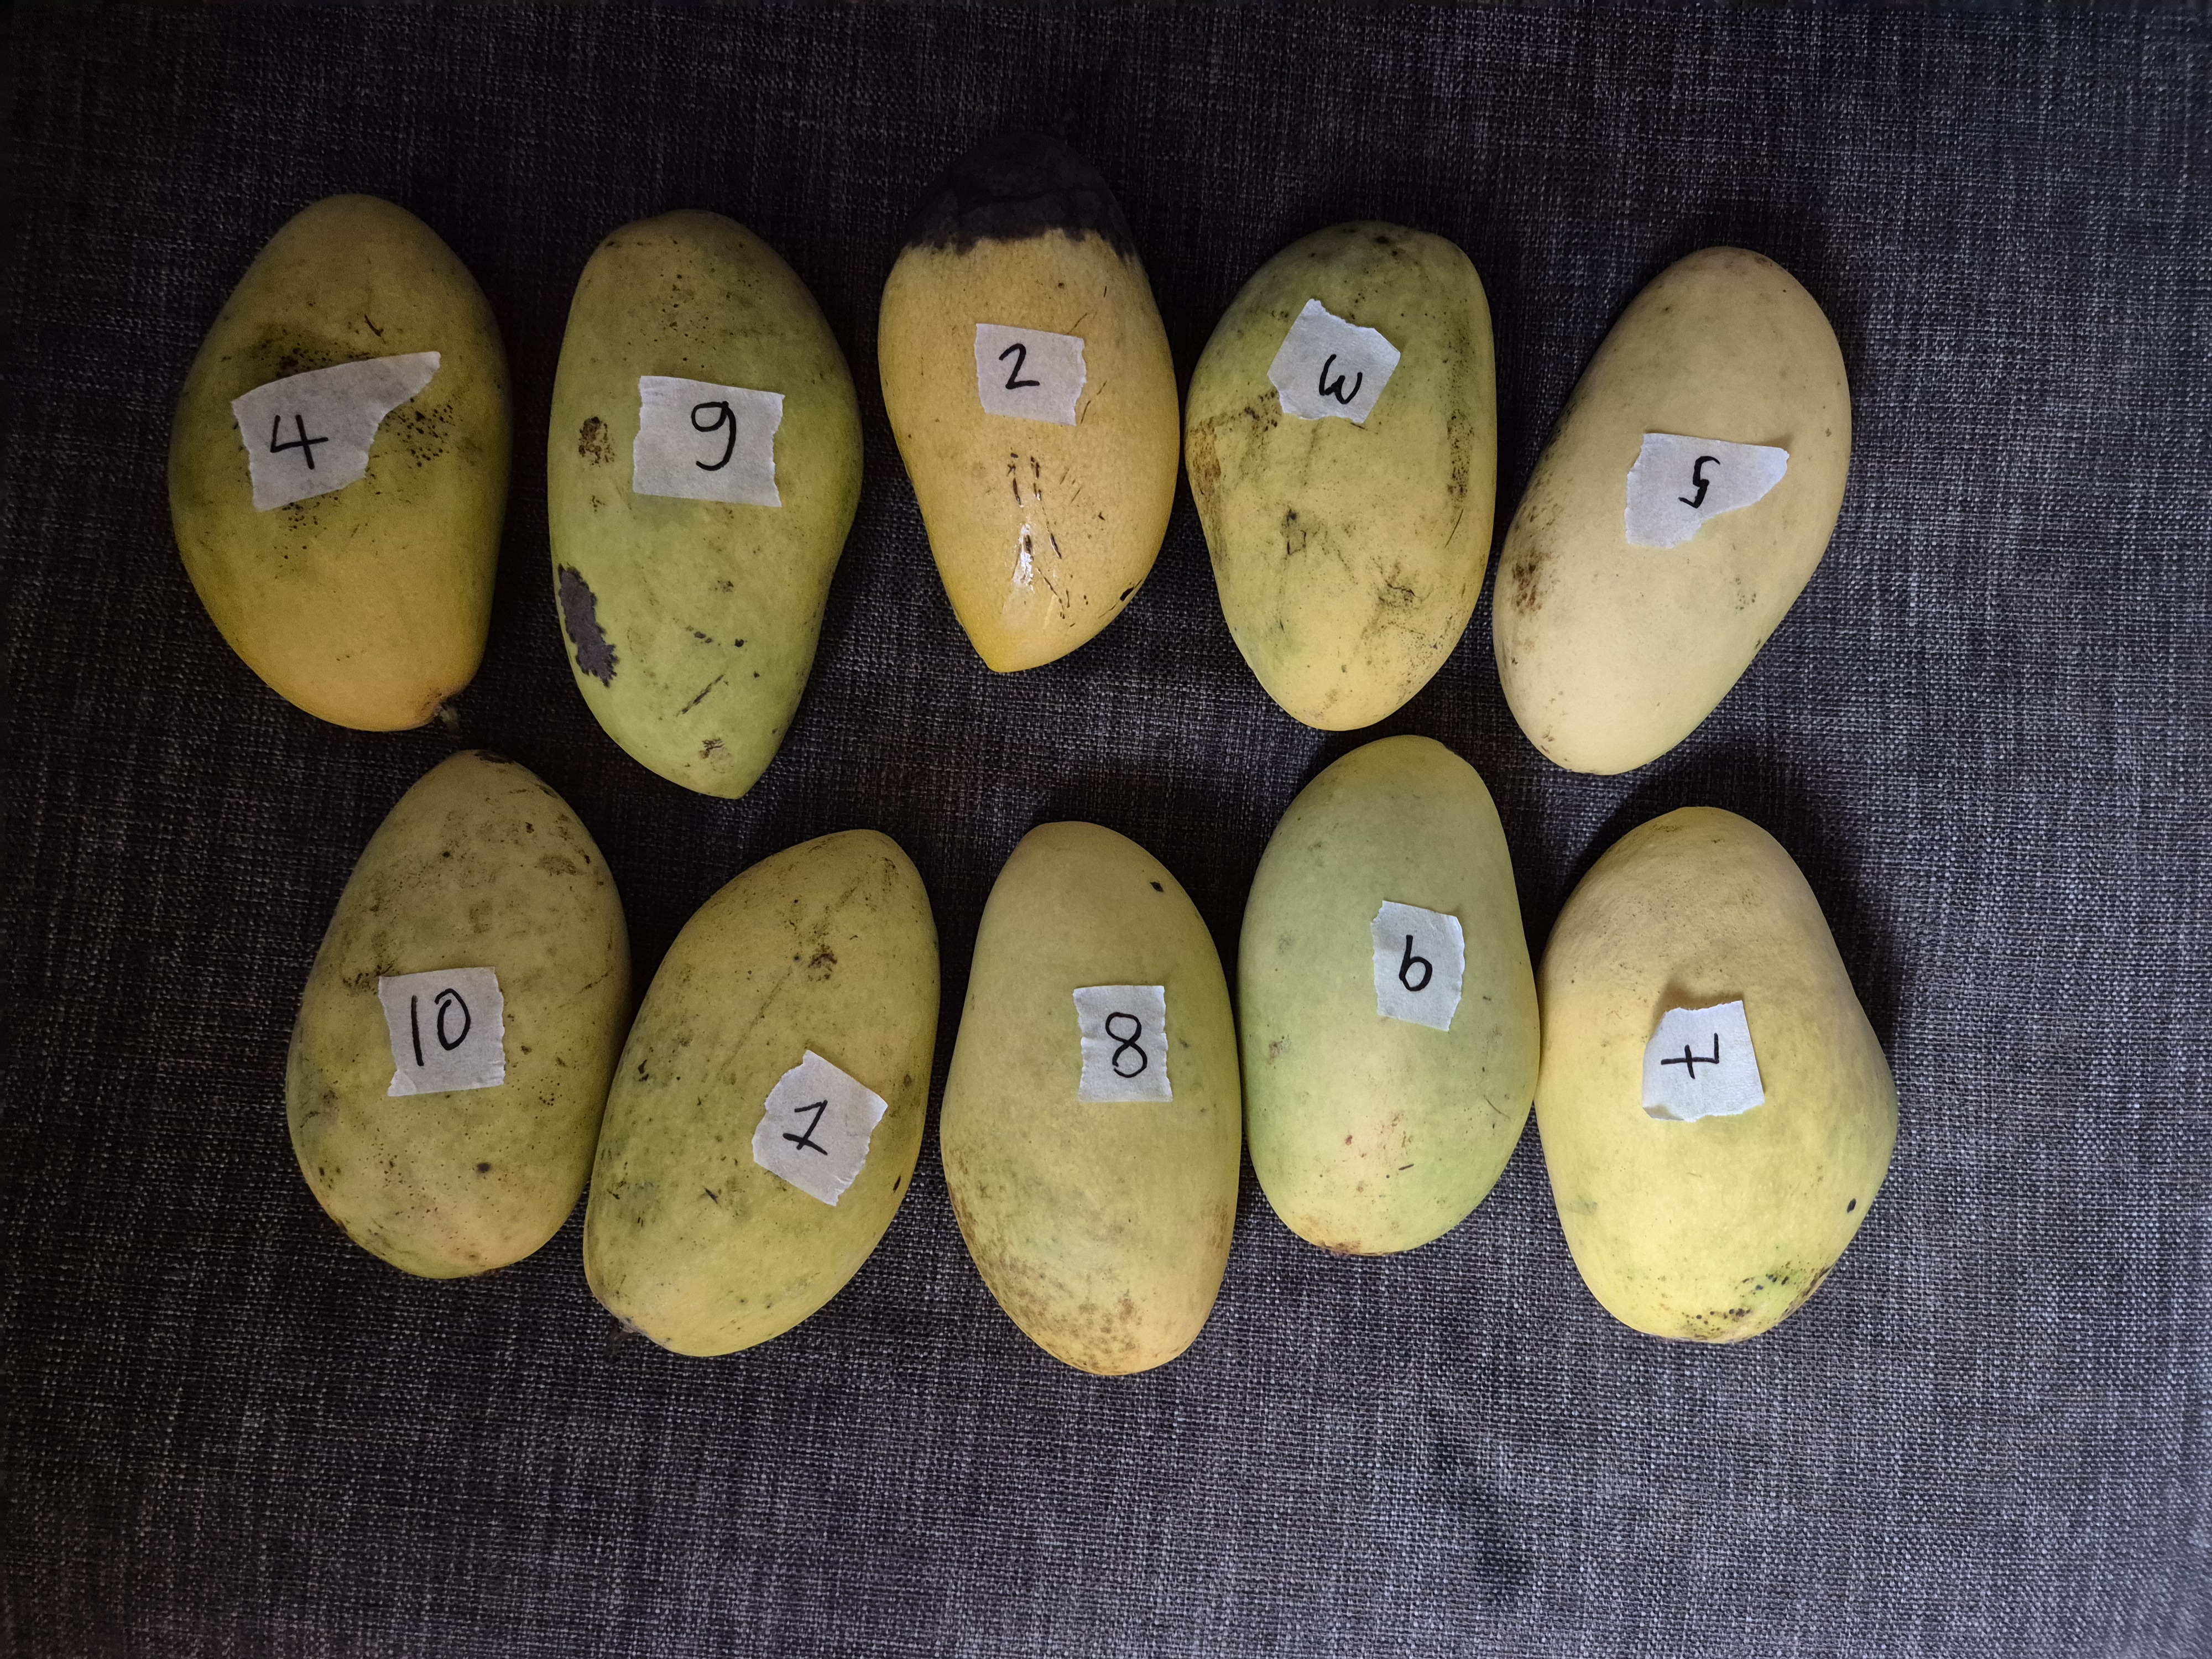
\includegraphics[width=0.45\textwidth]{/size-mango-test/ripe}
        \label{fig:ripe-mango}
    }
    \caption{Mangoes Tested for Size Measurement}
    \label{fig:mango_size_test}
\end{figure}

\begin{figure}[!htbp]
    \centering
    \subbottom[Original]{
        \includegraphics[width=0.45\textwidth]{/size-plots/Figure_1}
        \label{fig:m3_top}
    }
    \hfill
    \subbottom[Foreground Masking]{
        \includegraphics[width=0.45\textwidth]{/size-plots/Figure_2}
        \label{fig:m3_fm_top}
    }
    \vfill
    \subbottom[Background]{
        \includegraphics[width=0.45\textwidth]{/size-plots/Figure_3}
        \label{fig:m3_thresh_top}
    }
    \hfill
    \subbottom[Thresholding]{
        \includegraphics[width=0.45\textwidth]{/size-plots/Figure_4}
        \label{fig:m3_background}
    }
    \caption{Mango Top Side with White Conveyor}
    \label{fig:mango_3_top}
\end{figure}

\begin{figure}[!htbp]
    \centering
    \subbottom[Original]{
        \includegraphics[width=0.45\textwidth]{/size-plots/Figure_5}
        \label{fig:m3_top}
    }
    \hfill
    \subbottom[Foreground Masking]{
        \includegraphics[width=0.45\textwidth]{/size-plots/Figure_6}
        \label{fig:m3_fm_top}
    }
    \caption{Mango Top Side with White Conveyor}
    \label{fig:mango_3_top}
\end{figure}

\section{Formula with User Priority } \label{sec:userPriorityFormula}
\gls{not:bprio} and \gls{not:rprio} and \gls{not:sprio} are the \gls{User Priority-Based Grading} for bruises, ripeness, and size of the Carabao mango. 
Furthermore, \gls{not:bpred} and \gls{not:rpred} and \gls{not:spred} are the machine learning's predictions for bruises, ripeness, and size of the Carabao mango.
The formula for the user priority is given by:
\begin{equation}
	\label{eq:userPriority}	
  \text{Mango Grade} = \ensuremath{b \left( P \right)  B\left( P \right) + r \left( P \right) R\left( P \right) + s \left( P \right) S\left( P \right)}
\end{equation}

\noindent The machine learning predictions are assigned the following numerical values:

\subsection{Ripeness Scores:}
\begin{align}
r(\text{yellow}) &= 1.0 \\
r(\text{yellow\_green}) &= 2.0 \\
r(\text{green}) &= 3.0
\end{align}

\subsection{Bruises Scores:}
\begin{align}
b(\text{bruised}) &= 1.0 \\
b(\text{unbruised}) &= 2.0
\end{align}

\subsection{Size Scores:}
\begin{align}
s(\text{small}) &= 1.0 \\
s(\text{medium}) &= 2.0 \\
s(\text{large}) &= 3.0
\end{align}

% image of the coin
\begin{figure}[!htbp]
	\centering
	\includegraphics[width=0.8\textwidth]{/priority/bruises-only}
	\caption{Only Bruises as a None Zero Value}
	\label{fig:bruises-only-input}
\end{figure}

\begin{figure}[!htbp]
	\centering
	\includegraphics[width=0.8\textwidth]{/priority/ripeness-and-bruises-only}
	\caption{Only Ripeness and Bruises as a None Zero Value}
	\label{fig:ripeness-bruises-only-input}
\end{figure}

\begin{figure}[!htbp]
	\centering
	\includegraphics[width=0.8\textwidth]{/priority/ripeness-only}
	\caption{Only Ripeness as a None Zero Value}
	\label{fig:ripeness-only-input}
\end{figure}

\section{Physical Prototype} \label{sec:physicalPrototype}

Add pictures of the hardware prototype here with description

\begin{figure}[!htbp]
    \centering
    \subbottom[Prototype Top View]{
        \includegraphics[width=0.45\textwidth]{top_view}
        \label{fig:top_view}
    }
    \hfill
    \subbottom[Entrance Conveyor Belt View]{
        \includegraphics[width=0.45\textwidth]{side1}
        \label{fig:side1}
    }
    \vfill
    \subbottom[Side Conveyor Belt View]{
        \includegraphics[width=0.45\textwidth]{side2}
        \label{fig:side2}
    }
    \caption{Version 1: Prototype}
    \label{fig:v1_prototype}
\end{figure}

\begin{figure}[!htbp]
    \centering
    \subbottom[Prototype Main Hardware]{
        \includegraphics[width=0.45\textwidth]{schematic1}
        \label{fig:schematic1}
    }
    \hfill
    \subbottom[DC Motor and Pulley]{
        \includegraphics[width=0.45\textwidth]{DC_Motor_Pulley}
        \label{fig:dc_motor_pulley}
    }
    \vfill
    \subbottom[LED Lights and Camera Module]{
        \includegraphics[width=0.45\textwidth]{camera}
        \label{fig:camera}
    }
    \caption{Hardware View}
    \label{fig:hardware_view}
\end{figure}

\begin{figure}[!htbp]
    \centering
    \subbottom[Side View of Improved Prototype]{
        \includegraphics[width=0.45\textwidth]{new-side-view}
        \label{fig:new-side-view}
    }
    \hfill
    \subbottom[Top View of Improved Prototype]{
        \includegraphics[width=0.45\textwidth]{new-top-view}
        \label{fig:new-top-view}
    }
    \caption{Version 2: Improved Prototype}
    \label{fig:v2_prototype}
\end{figure}

\section{Software Application}

Show the raspberry pi app UI and demonstrate it here 

\begin{figure}[!htbp]
    \centering
    \subbottom[Version 1]{
        \includegraphics[width=0.45\textwidth]{UI_v1}
        \label{fig:ui_v1}
    }
    \hfill
    \subbottom[Version 2]{
        \includegraphics[width=0.45\textwidth]{UI_v2}
        \label{fig:ui_v2}
    }
    \vfill
    \subbottom[Version 3]{
        \includegraphics[width=0.45\textwidth]{UI_v3}
        \label{fig:ui_v3}
    }

    \caption{Version 1: User Interface of the Raspberry Pi}
    \label{fig:user_interface_v1}
\end{figure}

\begin{figure}[!htbp]
    \centering
    \subbottom[Version 2.1 with Background Image]{
        \includegraphics[width=0.45\textwidth]{/ui/ui-version1}
        \label{fig:app_v4}
    }
    \hfill
    \subbottom[Version 2.2 without Background Image]{
        \includegraphics[width=0.45\textwidth]{/ui/ui-version2}
        \label{fig:app_v5}
    }
    \caption{Version 2: User Interface of the Raspberry Pi}
    \label{fig:ui_main_v2}
\end{figure}

\begin{figure}[!htbp]
    \centering
    \subbottom[Version 1]{
        \includegraphics[width=0.45\textwidth]{sort_tree_1}
        \label{fig:sort_tree}
    }
    \hfill
    \subbottom[Version 2]{
        \includegraphics[width=0.45\textwidth]{sort_folder}
        \label{fig:sort_folder}
    }
    \vfill
    \subbottom[Version 3]{
        \includegraphics[width=0.45\textwidth]{sort_input_prior}
        \label{fig:input_folder_prior}
    }

    \caption{Mango Image Sorted}
    \label{fig:img_sorted}
\end{figure}

\begin{figure}[!htbp]
    \centering
    \subbottom[All Zero Error]{
        \includegraphics[width=0.45\textwidth]{/errors/all-zero}
        \label{fig:all-zero}
    }
    \hfill
    \subbottom[Input Error]{
        \includegraphics[width=0.45\textwidth]{/errors/input-error}
        \label{fig:input-error}
    }
    \vfill
    \subbottom[Null Button Error]{
        \includegraphics[width=0.45\textwidth]{/errors/null-button}
        \label{fig:null-button}
    }

    \caption{Error Messages}
    \label{fig:error-handel}
\end{figure}

\section{Summary} \label{sec:summary_results_and_discussions}

Provide the gist of this chapter such that it reflects the contents and the message. This is a compile test
\\

